\documentclass[12pt]{article}

\usepackage[utf8]{inputenc}
\usepackage[T1]{fontenc}
\usepackage[spanish]{babel}
\usepackage{graphicx}
\usepackage{xcolor}
\usepackage{geometry}
\usepackage{amsmath, amssymb}
\usepackage{ragged2e}
\usepackage{tikz}
\usetikzlibrary{positioning}

\geometry{margin=2.5cm}
\setlength{\parskip}{0.8em}
\setlength{\parindent}{0pt}

\begin{document}
	
	\begin{flushleft}
		\begin{minipage}{0.8\textwidth}
			\begin{minipage}[c]{0.50\textwidth}
				\includegraphics[width=\textwidth]{img/unalB.pdf}
			\end{minipage}
			\hspace{1em}%
			\raisebox{-4.7em}{\textcolor{gray}{\vrule width 1pt height 10em}}%
			\hspace{1.9em}%
			\begin{minipage}[c]{0.75\textwidth}
				\raggedright
				Sede Manizales\\
				Taller 6: Estrategias voraces
				\\[0.3em]
				\textbf{Integrantes:}\\
				Santiago Marín Giraldo\\
				Tomás Henao Bonilla
			\end{minipage}
		\end{minipage}
	\end{flushleft}
	
	\section*{Problema I}
	
	Dibuje la secuencia de grafos que muestre cómo progresa el algoritmo de \textbf{Prim}, en cada paso, al calcular el árbol generador de peso mínimo para el siguiente grafo, tomando como nodo raíz el 1:
	
	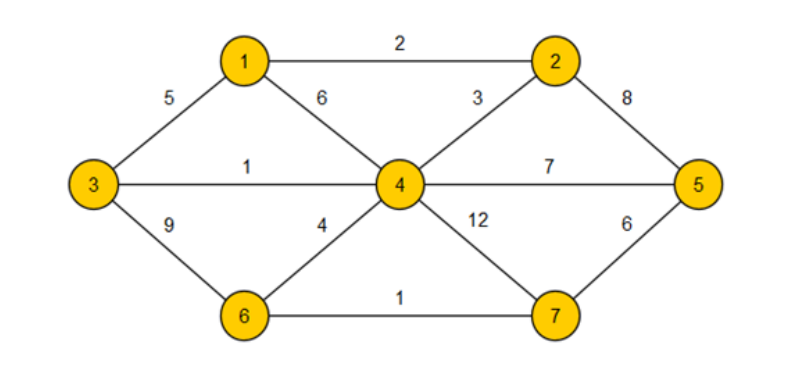
\includegraphics[width=\textwidth]{img/Grafo 1}
	
	\subsection*{Paso 1}
	
	Iniciamos desde el nodo 1, en donde se nos presentan las siguientes aristas disponibles:
	\[(1,2)=2,\quad (1,3)=5,\quad (1,4)=6\]
	
	Se selecciona la arista de menor peso:
	\[(1,2)=2\]
	
	\begin{center}
		\begin{tikzpicture}[scale=1.2]
			\node[circle,draw,fill=yellow!60] (1) at (0,0) {1};
			\node[circle,draw,fill=yellow!60] (2) at (3,0) {2};
			\draw[thick] (1)-- node[above]{2} (2);
		\end{tikzpicture}
	\end{center}
	
	Obteniendo así el conjunto actual de la forma:
	\[\{1,2\}\]
	
	\subsection*{Paso 2}
	
	Ahora poseemos las siguientes aristas disponibles:
	\[(1,3)=5,\quad (1,4)=6,\quad (2,4)=3,\quad (2,5)=8\]
	
	Se selecciona la arista de menor peso:
	\[(2,4)=3\]
	
	\begin{center}
		\begin{tikzpicture}[scale=1.2]
			
			\node[circle,draw,fill=yellow!60] (1) at (0,0) {1};
			\node[circle,draw,fill=yellow!60] (2) at (3,0) {2};
			\node[circle,draw,fill=yellow!60] (4) at (6,0) {4};
			
			\draw[thick] (1)-- node[above]{2} (2);
			\draw[thick] (2)-- node[above]{3} (4);
			
		\end{tikzpicture}
	\end{center}
	
	Actualizamos el conjunto:
	\[\{1,2,4\}\]
	
	\subsection*{Paso 3}
	
	Ahora poseemos las siguientes aristas disponibles:
	\[(1,3)=5,\quad (4,3)=1,\quad (4,6)=4,\quad (4,5)=7\]
	
	Se selecciona la arista de menor peso:
	\[(4,3)=1\]
	
	\begin{center}
		\begin{tikzpicture}[scale=1.2]
			
			\node[circle,draw,fill=yellow!60] (1) at (0,0) {1};
			\node[circle,draw,fill=yellow!60] (2) at (3,0) {2};
			\node[circle,draw,fill=yellow!60] (4) at (6,0) {4};
			\node[circle,draw,fill=yellow!60] (3) at (6,-2) {3};
			
			\draw[thick] (1)-- node[above]{2} (2);
			\draw[thick] (2)-- node[above]{3} (4);
			\draw[thick] (4)-- node[right]{1} (3);
			
		\end{tikzpicture}
	\end{center}
	
	Actualizamos el conjunto:
	\[\{1,2,3,4\}\]
	
	\subsection*{Paso 4}
	
	Ahora poseemos las siguientes aristas disponibles:
	\[(4,6)=4,\quad (4,5)=7,\quad (2,5)=8,\quad (3,6)=9\]
	
	Se selecciona la arista de menor peso:
	\[(4,6)=4\]
	
	\begin{center}
		\begin{tikzpicture}[scale=1.2]
			
			\node[circle,draw,fill=yellow!60] (1) at (0,0) {1};
			\node[circle,draw,fill=yellow!60] (2) at (3,0) {2};
			\node[circle,draw,fill=yellow!60] (4) at (6,0) {4};
			\node[circle,draw,fill=yellow!60] (3) at (6,-2) {3};
			\node[circle,draw,fill=yellow!60] (6) at (9,0) {6};
			
			\draw[thick] (1)-- node[above]{2} (2);
			\draw[thick] (2)-- node[above]{3} (4);
			\draw[thick] (4)-- node[left]{1} (3);
			\draw[thick] (4)-- node[above]{4} (6);
			
		\end{tikzpicture}
	\end{center}
	
	Actualizamos el conjunto:
	\[\{1,2,3,4,6\}\]
	
	\subsection*{Paso 5}
	
	Ahora poseemos las siguientes aristas disponibles:
	\[(6,7)=1,\quad (4,5)=7,\quad (2,5)=8\]
	
	Se selecciona la arista de menor peso:
	\[(6,7)=1\]
	
	\begin{center}
		\begin{tikzpicture}[scale=1.2]
			
			\node[circle,draw,fill=yellow!60] (1) at (0,0) {1};
			\node[circle,draw,fill=yellow!60] (2) at (3,0) {2};
			\node[circle,draw,fill=yellow!60] (4) at (6,0) {4};
			\node[circle,draw,fill=yellow!60] (3) at (6,-2) {3};
			\node[circle,draw,fill=yellow!60] (6) at (9,0) {6};
			\node[circle,draw,fill=yellow!60] (7) at (12,0) {7};
			
			\draw[thick] (1)-- node[above]{2} (2);
			\draw[thick] (2)-- node[above]{3} (4);
			\draw[thick] (4)-- node[left]{1} (3);
			\draw[thick] (4)-- node[above]{4} (6);
			\draw[thick] (6)-- node[above]{1} (7);
			
		\end{tikzpicture}
	\end{center}
	
	Conjunto actual:
	\[\{1,2,3,4,6,7\}\]
	
	\subsection*{Paso 6}
	
	Ahora poseemos las siguientes aristas disponibles:
	\[(7,5)=6,\quad (4,5)=7,\quad (2,5)=8\]
	
	Se selecciona la arista de menor peso:
	\[(7,5)=6\]
	
	\begin{center}
		\begin{tikzpicture}[scale=1.2]
			
			\node[circle,draw,fill=yellow!60] (1) at (0,0) {1};
			\node[circle,draw,fill=yellow!60] (2) at (3,0) {2};
			\node[circle,draw,fill=yellow!60] (4) at (6,0) {4};
			\node[circle,draw,fill=yellow!60] (3) at (6,-2) {3};
			\node[circle,draw,fill=yellow!60] (6) at (9,0) {6};
			\node[circle,draw,fill=yellow!60] (7) at (12,0) {7};
			\node[circle,draw,fill=yellow!60] (5) at (15,0) {5};
			
			\draw[thick] (1)-- node[above]{2} (2);
			\draw[thick] (2)-- node[above]{3} (4);
			\draw[thick] (4)-- node[left]{1} (3);
			\draw[thick] (4)-- node[above]{4} (6);
			\draw[thick] (6)-- node[above]{1} (7);
			\draw[thick] (7)-- node[above]{6} (5);
			
		\end{tikzpicture}
	\end{center}
	
	\subsection*{Árbol generador mínimo}
	
	Las aristas seleccionadas fueron:
	\[\{(1,2),(2,4),(4,3),(4,6),(6,7),(7,5)\}\]
	
	Peso total:
	\[2+3+1+4+1+6 = 17\]
	
	\[\boxed{Peso\ total = 17}\]
	
	Podemos concluir que, mediante la implementación del algoritmo de \textbf{Prim}, se logró construir el árbol generador mínimo del grafo. El árbol obtenido conecta todos los vértices mediante las aristas de menor peso posible sin formar ciclos, obteniendo un peso mínimo total de 17.
	
	\section*{Problema II}       
	
	Dibuje la secuencia de grafos que muestre cómo progresa el algoritmo de \textbf{Kruskal}, en cada paso, al calcular el árbol
	generador de peso mínimo para el grafo del punto 1.
	
	
	El algoritmo de \textbf{Kruskal} es un algoritmo voraz utilizado para encontrar el árbol generador mínimo de un grafo conectado y ponderado. Su funcionamiento consiste en ordenar todas las aristas del grafo de menor a mayor peso e ir seleccionándolas progresivamente, siempre que no formen ciclos. El proceso continúa hasta conectar todos los vértices del grafo con el menor costo total posible, obteniendo así un árbol generador mínimo.
	

	\subsection*{Paso 1}
	
	Ordenamos las aristas del grafo de menor a mayor peso y seleccionamos la primera arista disponible:\[(3,4)=1\]
	
	\begin{center}
		\begin{tikzpicture}[scale=1.2]
			
			\node[circle,draw,fill=yellow!60] (1) at (2,4) {1};
			\node[circle,draw,fill=yellow!60] (2) at (6,4) {2};
			\node[circle,draw,fill=yellow!60] (3) at (0,2) {3};
			\node[circle,draw,fill=yellow!60] (4) at (4,2) {4};
			\node[circle,draw,fill=yellow!60] (5) at (8,2) {5};
			\node[circle,draw,fill=yellow!60] (6) at (2,0) {6};
			\node[circle,draw,fill=yellow!60] (7) at (6,0) {7};
			
			\draw[thick] (3)-- node[above]{1} (4);
			
		\end{tikzpicture}
	\end{center}
	
	\subsection*{Paso 2}
	
	La siguiente arista de menor peso es: \[(6,7)=1\]
	
	\begin{center}
		\begin{tikzpicture}[scale=1.2]
			
			\node[circle,draw,fill=yellow!60] (1) at (2,4) {1};
			\node[circle,draw,fill=yellow!60] (2) at (6,4) {2};
			\node[circle,draw,fill=yellow!60] (3) at (0,2) {3};
			\node[circle,draw,fill=yellow!60] (4) at (4,2) {4};
			\node[circle,draw,fill=yellow!60] (5) at (8,2) {5};
			\node[circle,draw,fill=yellow!60] (6) at (2,0) {6};
			\node[circle,draw,fill=yellow!60] (7) at (6,0) {7};
			
			\draw[thick] (3)-- node[above]{1} (4);
			\draw[thick] (6)-- node[below]{1} (7);
			
		\end{tikzpicture}
	\end{center}
	
	\subsection*{Paso 3}
	
	La siguiente arista de menor peso es: \[(1,2)=2\]
	
	\begin{center}
		\begin{tikzpicture}[scale=1.2]
			
			\node[circle,draw,fill=yellow!60] (1) at (2,4) {1};
			\node[circle,draw,fill=yellow!60] (2) at (6,4) {2};
			\node[circle,draw,fill=yellow!60] (3) at (0,2) {3};
			\node[circle,draw,fill=yellow!60] (4) at (4,2) {4};
			\node[circle,draw,fill=yellow!60] (5) at (8,2) {5};
			\node[circle,draw,fill=yellow!60] (6) at (2,0) {6};
			\node[circle,draw,fill=yellow!60] (7) at (6,0) {7};
			
			\draw[thick] (3)-- node[above]{1} (4);
			\draw[thick] (6)-- node[below]{1} (7);
			\draw[thick] (1)-- node[above]{2} (2);
			
		\end{tikzpicture}
	\end{center}
	
	\subsection*{Paso 4}
	
	La siguiente arista de menor peso es: \[(2,4)=3\]
	
	\begin{center}
		\begin{tikzpicture}[scale=1.2]
			
			\node[circle,draw,fill=yellow!60] (1) at (2,4) {1};
			\node[circle,draw,fill=yellow!60] (2) at (6,4) {2};
			\node[circle,draw,fill=yellow!60] (3) at (0,2) {3};
			\node[circle,draw,fill=yellow!60] (4) at (4,2) {4};
			\node[circle,draw,fill=yellow!60] (5) at (8,2) {5};
			\node[circle,draw,fill=yellow!60] (6) at (2,0) {6};
			\node[circle,draw,fill=yellow!60] (7) at (6,0) {7};
			
			\draw[thick] (3)-- node[above]{1} (4);
			\draw[thick] (6)-- node[below]{1} (7);
			\draw[thick] (1)-- node[above]{2} (2);
			\draw[thick] (2)-- node[right]{3} (4);
			
		\end{tikzpicture}
	\end{center}
	
	\subsection*{Paso 5}
	
	La siguiente arista de menor peso es: \[(4,6)=4\]
	
	\begin{center}
		\begin{tikzpicture}[scale=1.2]
			
			\node[circle,draw,fill=yellow!60] (1) at (2,4) {1};
			\node[circle,draw,fill=yellow!60] (2) at (6,4) {2};
			\node[circle,draw,fill=yellow!60] (3) at (0,2) {3};
			\node[circle,draw,fill=yellow!60] (4) at (4,2) {4};
			\node[circle,draw,fill=yellow!60] (5) at (8,2) {5};
			\node[circle,draw,fill=yellow!60] (6) at (2,0) {6};
			\node[circle,draw,fill=yellow!60] (7) at (6,0) {7};
			
			\draw[thick] (3)-- node[above]{1} (4);
			\draw[thick] (6)-- node[below]{1} (7);
			\draw[thick] (1)-- node[above]{2} (2);
			\draw[thick] (2)-- node[right]{3} (4);
			\draw[thick] (4)-- node[left]{4} (6);
			
		\end{tikzpicture}
	\end{center}
	
	\subsection*{Paso 6}
	
	La siguiente arista válida de menor peso es: \[(7,5)=6\]
	
	\begin{center}
		\begin{tikzpicture}[scale=1.2]
			
			\node[circle,draw,fill=yellow!60] (1) at (2,4) {1};
			\node[circle,draw,fill=yellow!60] (2) at (6,4) {2};
			\node[circle,draw,fill=yellow!60] (3) at (0,2) {3};
			\node[circle,draw,fill=yellow!60] (4) at (4,2) {4};
			\node[circle,draw,fill=yellow!60] (5) at (8,2) {5};
			\node[circle,draw,fill=yellow!60] (6) at (2,0) {6};
			\node[circle,draw,fill=yellow!60] (7) at (6,0) {7};
			
			\draw[thick] (3)-- node[above]{1} (4);
			\draw[thick] (6)-- node[below]{1} (7);
			\draw[thick] (1)-- node[above]{2} (2);
			\draw[thick] (2)-- node[right]{3} (4);
			\draw[thick] (4)-- node[left]{4} (6);
			\draw[thick] (7)-- node[right]{6} (5);
			
		\end{tikzpicture}
	\end{center}
	
	\subsection*{Árbol generador mínimo}
	
	Las aristas seleccionadas fueron:
	\[\{(3,4),(6,7),(1,2),(2,4),(4,6),(7,5)\}\]
	
	Peso total:
	\[1+1+2+3+4+6 = 17\]
	
	\[\boxed{Peso\ total = 17}\]
	
	Podemos decir que, mediante la implementación del algoritmo de \textbf{Kruskal}, se logró construir el árbol generador mínimo del grafo seleccionando las aristas de menor peso posible sin formar ciclos. El árbol obtenido conecta todos los vértices y presenta un peso mínimo total de 17.
	

	\section*{Problema III}
	
	Para el algoritmo de \textbf{Prim} se pueden identificar las siguientes funciones características de los algoritmos voraces:
	
	\subsection*{(i) Función objetivo}
	
	La función objetivo del algoritmo consiste en construir un árbol generador mínimo, buscando que la suma total de los pesos de las aristas seleccionadas sea la menor posible. De esta manera, se logra conectar todos los vértices del grafo con el costo mínimo.
	
	\subsection*{(ii) Función de selección}
	
	En cada iteración, el algoritmo selecciona la arista de menor peso que conecte un vértice que ya pertenece al árbol con otro vértice que todavía no haya sido incluido. Esta selección se realiza de forma voraz, escogiendo siempre la opción más económica disponible.
	
	\subsection*{(iii) Función de factibilidad}
	
	La función de factibilidad verifica que la arista seleccionada pueda agregarse al árbol sin formar ciclos. Además, debe permitir incorporar un nuevo vértice al conjunto de vértices ya conectados.
	
	\subsection*{(iv) Función solución}
	
	La solución se alcanza cuando todos los vértices del grafo han sido conectados y el árbol generador contiene exactamente \(n-1\) aristas, donde \(n\) representa el número total de vértices del grafo.

	\section*{Problema IV}
	
	Se dispone de una única sala y un conjunto de \(n\) reuniones 
	\[A = \{1,\ldots,n\}\] Cada reunión \(k\) tiene hora de inicio \(s_k\) y hora de finalización \(f_k\) con \(s_k < f_k\).
	
	Dos reuniones no pueden solaparse en el tiempo, es decir, no pueden usar simultáneamente la sala.

	hola mundo el santi


	
	 
\end{document}